% This file was created by matplotlib2tikz v0.7.4.
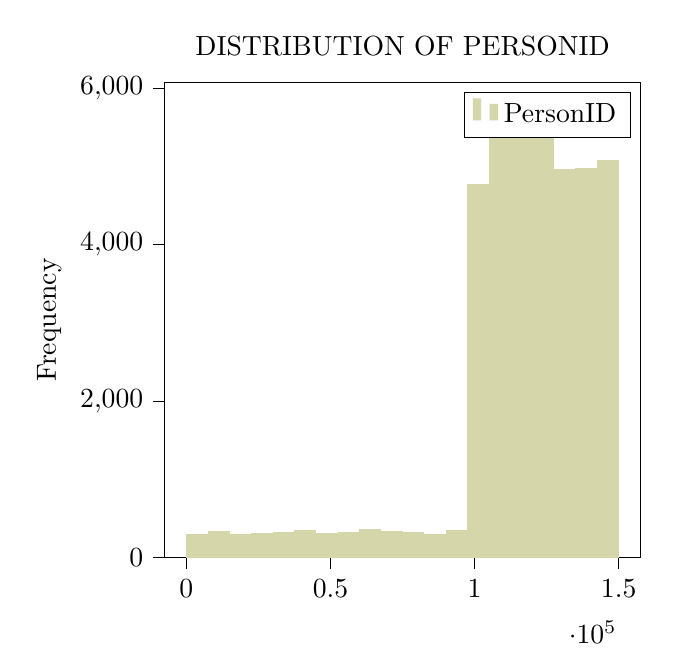
\begin{tikzpicture}

\definecolor{color0}{rgb}{0.835294117647059,0.83921568627451,0.666666666666667}

\begin{axis}[
height=3in,
tick align=outside,
tick pos=left,
title={\printsubsection{\MakeUppercase{Distribution of PersonID}}\\},
width=3in,
x grid style={white!69.01960784313725!black},
xmin=-7476.85, xmax=157497.85,
xtick style={color=black},
y grid style={white!69.01960784313725!black},
ylabel={Frequency},
ymin=0, ymax=6073.2,
ytick style={color=black}
]
\draw[fill=color0,draw opacity=0] (axis cs:22,0) rectangle (axis cs:7520.85,300);
\addlegendimage{ybar,ybar legend,fill=color0,draw opacity=0};
\addlegendentry{PersonID}

\draw[fill=color0,draw opacity=0] (axis cs:7520.85,0) rectangle (axis cs:15019.7,340);
\draw[fill=color0,draw opacity=0] (axis cs:15019.7,0) rectangle (axis cs:22518.55,304);
\draw[fill=color0,draw opacity=0] (axis cs:22518.55,0) rectangle (axis cs:30017.4,310);
\draw[fill=color0,draw opacity=0] (axis cs:30017.4,0) rectangle (axis cs:37516.25,334);
\draw[fill=color0,draw opacity=0] (axis cs:37516.25,0) rectangle (axis cs:45015.1,357);
\draw[fill=color0,draw opacity=0] (axis cs:45015.1,0) rectangle (axis cs:52513.95,310);
\draw[fill=color0,draw opacity=0] (axis cs:52513.95,0) rectangle (axis cs:60012.8,328);
\draw[fill=color0,draw opacity=0] (axis cs:60012.8,0) rectangle (axis cs:67511.65,362);
\draw[fill=color0,draw opacity=0] (axis cs:67511.65,0) rectangle (axis cs:75010.5,341);
\draw[fill=color0,draw opacity=0] (axis cs:75010.5,0) rectangle (axis cs:82509.35,329);
\draw[fill=color0,draw opacity=0] (axis cs:82509.35,0) rectangle (axis cs:90008.2,303);
\draw[fill=color0,draw opacity=0] (axis cs:90008.2,0) rectangle (axis cs:97507.05,350);
\draw[fill=color0,draw opacity=0] (axis cs:97507.05,0) rectangle (axis cs:105005.9,4772);
\draw[fill=color0,draw opacity=0] (axis cs:105005.9,0) rectangle (axis cs:112504.75,5784);
\draw[fill=color0,draw opacity=0] (axis cs:112504.75,0) rectangle (axis cs:120003.6,5764);
\draw[fill=color0,draw opacity=0] (axis cs:120003.6,0) rectangle (axis cs:127502.45,5408);
\draw[fill=color0,draw opacity=0] (axis cs:127502.45,0) rectangle (axis cs:135001.3,4962);
\draw[fill=color0,draw opacity=0] (axis cs:135001.3,0) rectangle (axis cs:142500.15,4975);
\draw[fill=color0,draw opacity=0] (axis cs:142500.15,0) rectangle (axis cs:149999,5083);
\end{axis}

\end{tikzpicture}